\documentclass[xcolor=x11names,compress]{beamer}

%% General document %%%%%%%%%%%%%%%%%%%%%%%%%%%%%%%%%%
\usepackage{graphicx}
\usepackage{tikz}
\usepackage{Tabbing}
\usetikzlibrary{decorations.fractals}
\usepackage{fancyvrb}
%%%%%%%%%%%%%%%%%%%%%%%%%%%%%%%%%%%%%%%%%%%%%%%%%%%%%%

%% Beamer Layout %%%%%%%%%%%%%%%%%%%%%%%%%%%%%%%%%%
\useoutertheme[subsection=false,shadow]{miniframes}
\useinnertheme{default}
\usefonttheme{serif}
\usepackage{palatino}
\usepackage{tabu}
% Links
\usepackage{hyperref}
\definecolor{links}{HTML}{003262}
\hypersetup{colorlinks,linkcolor=,urlcolor=links}

% addition of color
\usepackage{xcolor}
\definecolor{CoolBlack}{rgb}{0.0, 0.18, 0.39}
\definecolor{byellow}{rgb}{0.55037, 0.38821, 0.06142}
\definecolor{dgreen}{rgb}{0.,0.6,0.}
\definecolor{RawSienna}{cmyk}{0,0.72,1,0.45}
\definecolor{forestgreen(web)}{rgb}{0.13, 0.55, 0.13}
\definecolor{cardinal}{rgb}{0.77, 0.12, 0.23}

\setbeamerfont{title like}{shape=\scshape}
\setbeamerfont{frametitle}{shape=\scshape}

\setbeamercolor*{lower separation line head}{bg=CoolBlack} 
\setbeamercolor*{normal text}{fg=black,bg=white} 
\setbeamercolor*{alerted text}{fg=dgreen} % just testing; I think this looks better
\setbeamercolor*{example text}{fg=black} 
\setbeamercolor*{structure}{fg=black} 
 
\setbeamercolor*{palette tertiary}{fg=black,bg=black!10} 
\setbeamercolor*{palette quaternary}{fg=black,bg=black!10} 

% Margins
\usepackage{changepage}

\mode<presentation>
{
  \definecolor{berkeleyblue}{HTML}{003262}
  \definecolor{berkeleygold}{HTML}{FDB515}
  \usetheme{Boadilla}      % or try Darmstadt, Madrid, Warsaw, Boadilla...
  %\usecolortheme{dove} % or try albatross, beaver, crane, ...
  \setbeamercolor{structure}{fg=berkeleyblue,bg=berkeleygold}
  \setbeamercolor{palette primary}{bg=berkeleyblue,fg=white} % changed this
  \setbeamercolor{palette secondary}{fg=berkeleyblue,bg=berkeleygold} % changed this
  \setbeamercolor{palette tertiary}{bg=berkeleyblue,fg=white} % changed this
  \usefonttheme{structurebold}  % or try serif, structurebold, ...
  \useinnertheme{circles}
  \setbeamertemplate{navigation symbols}{}
  \setbeamertemplate{caption}[numbered]
  \usebackgroundtemplate{}
}

% Columns
\renewcommand{\(}{\begin{columns}}
\renewcommand{\)}{\end{columns}}
\newcommand{\<}[1]{\begin{column}{#1}}
\renewcommand{\>}{\end{column}}

\usepackage{cutwin}

% adding slide numbers
\addtobeamertemplate{navigation symbols}{}{%
    \usebeamerfont{footline}%
    \usebeamercolor[fg]{footline}%
    \hspace{1em}%
    \insertframenumber/\inserttotalframenumber
}

% equation stuff
\newcommand{\Macro}{\ensuremath{\Sigma}}
\newcommand{\Sn}{\ensuremath{S_N} }
\newcommand{\vOmega}{\ensuremath{\hat{\Omega}}}
\usepackage{mathrsfs}
\usepackage[mathcal]{euscript}
\usepackage{amssymb}
\usepackage{amsthm}
\usepackage{epsfig}
\usepackage{amsmath}
\newcommand{\ve}[1]{\ensuremath{\mathbf{#1}}}
\newcommand{\micro}{\ensuremath{\sigma}}
\newcommand{\detR}{\ensuremath{\Sigma}}

% title stuff for footer
\title{Approaches to HPC in NE}
\author{R.\ N.\ Slaybaugh}
\date{8 December 2014}

%%%%%%%%%%%%%%%%%%%%%%%%%%%%%%%%%%%%%%%%%%%%%%%%%%%%%%
\begin{document}

%%%%%%%%%%%%%%%%%%%%%%%%%%%%%%%%%%%%%%%%%%%%%%%%%%%%%%
\begin{frame}
\title{Advanced Approaches to High-Performance Computing in Nuclear:}
\subtitle{Applications to Non-Proliferation}
\author{\includegraphics[height=2cm]{../bk-eps-converted-to}\\R.\ N.\ Slaybaugh \\ Univ.\ of Cal.\ Berkeley}

\date{MIIT Delegation VISIT to BNRC \\ 8 December 2014}
\titlepage
\end{frame}

%------------------------------------------------------
\begin{frame}{What Are We Sovling?}

    My group studies how to solve the steady state, neutral particle Boltzmann
    transport equation more efficiently:
    %   
    \begin{align}
    [\vOmega \cdot \nabla + \Macro(\vec{r}, E)] &\psi(\vec{r}, \vOmega, E)  =  q(\vec{r}, \vOmega, E) + \nonumber\\
     &\int_0^{\infty} dE' \int_{4\pi} d\vOmega' \:\Macro_{s}(\vec{r}, E' \to E,
     \vOmega' \cdot \vOmega) \psi(\vec{r}, \vOmega', E') \nonumber
    \end{align}
    
    \begin{columns}
    \begin{column}{0.55\textwidth}     
 	   \begin{center}
 	   \begin{figure}
 	   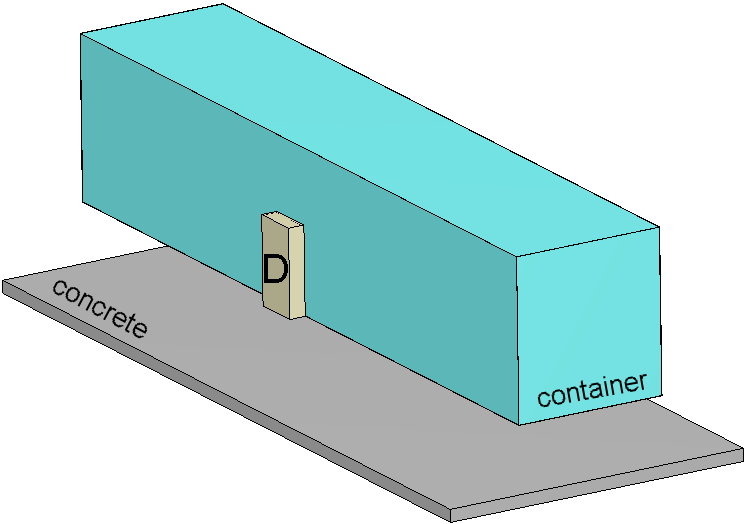
\includegraphics[height=1.5in,clip]{../figs/cargo-container}
       \end{figure}
 	   \end{center}
  	\end{column}
   	%
 	\begin{column}{0.4\textwidth}
 	   \begin{center}
 	   \begin{figure}     
 	   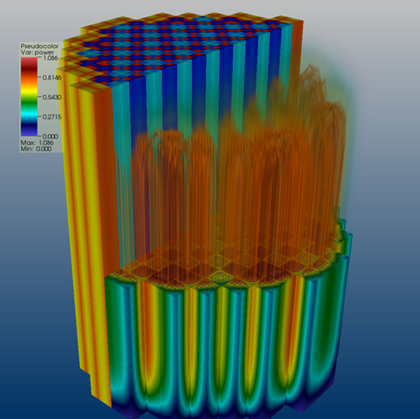
\includegraphics[height=1.5in,clip]{../figs/denovo-pwr}
 	   \end{figure}
 	   \end{center}
  	\end{column}
    \end{columns}
   
\end{frame}

%------------------------------------------------------
\begin{frame}{How Do We Solve It?}
    
    \begin{itemize}
    \item \alert{Deterministic} methods require discretization of phase space
      \begin{itemize}
      \item discretize more finely to improve solution quality
      \item use advanced solvers to converge solution more quickly
      \end{itemize}
      %
      \begin{align}
      \mathbf{L} \psi &= \mathbf{MS}\phi + \mathbf{Q} \nonumber\\
      \phi &= \mathbf{D}\psi \nonumber \\
      \underbrace{(\ve{I} - \ve{DL}^{-1}\ve{MS})}_{\mathbf{A}}\phi &= q\nonumber
      \end{align}
      %        
    \item \alert{Monte Carlo} (MC) treats phase space continuously
      \begin{itemize}
      \item accuracy depends on number of particles simulated
      \item often requires variance reduction (VR)
      \end{itemize}      
    \item \alert{Hybrid} methods: create MC VR parameters using deterministic solutions
    \end{itemize}
    
\end{frame}

% ------------------------------------------------------
\begin{frame}{What Drives the Challenges and Solutions?}
    	
    	\alert{Data} determines matrix properties, memory needs, and solution flow
    	
    \begin{columns}
    \begin{column}{0.55\textwidth}     
 	   \begin{center}
 	   \begin{figure}
 	   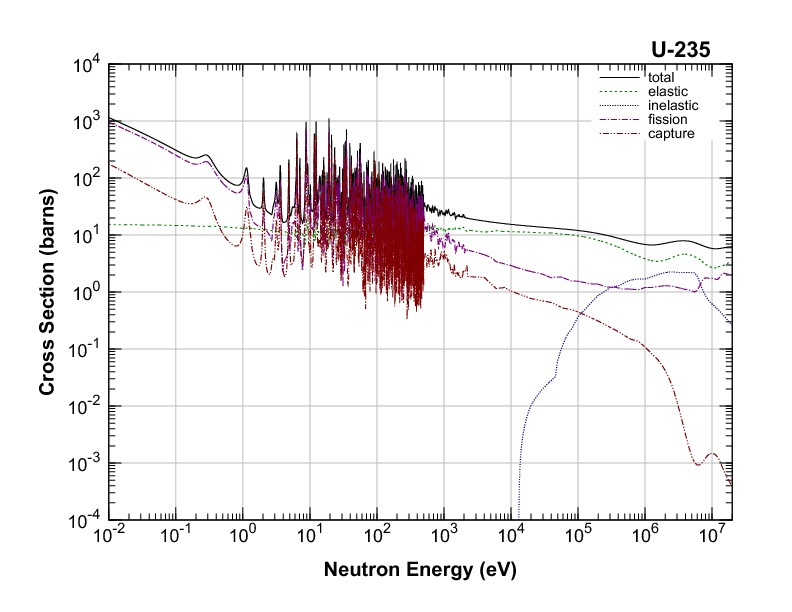
\includegraphics[height=2.25in,clip]{../figs/u235-xsecs}
       \end{figure}
 	   \end{center}
  	\end{column}
   	%
 	\begin{column}{0.4\textwidth}
 	   \begin{center}
 	   \begin{figure}     
 	   \includegraphics[height=1.25in, width=1.25in, clip]{../figs/Fe-D2O-C-space-energy}
 	   %Evans
 	   \end{figure}
 	   \begin{figure} 
 	   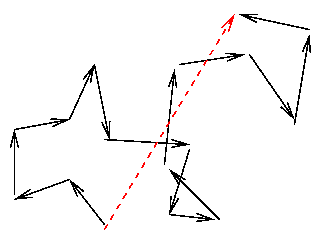
\includegraphics[height=1in,clip]{../figs/random-walk}
       \end{figure}
 	   \end{center}
  	\end{column}
	\end{columns}
	
\end{frame}

%------------------------------------------------------
\begin{frame}{What Drives the Challenges and Solutions?}
    
    \begin{columns}
    \begin{column}{0.3\textwidth}
 	   \begin{center}
 	   \begin{figure}     
 	   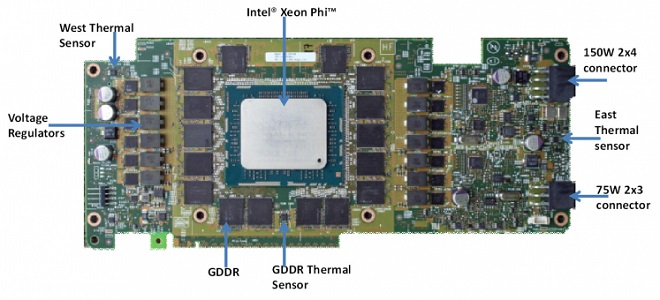
\includegraphics[height=1.25in,clip]{../figs/Intel-Xeon-Phi-Board}
 	   \end{figure}
 	   \end{center}
    \end{column}
   	%
 	\begin{column}{0.8\textwidth}
 	   \begin{center}
 	   \begin{figure} 
 	   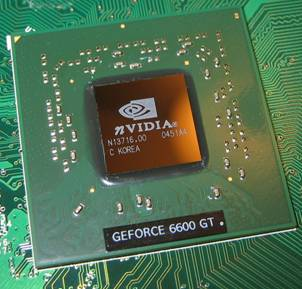
\includegraphics[height=1in,clip]{../figs/GPU}
       \end{figure}
 	   \end{center}
  	\end{column}
	\end{columns}
	
	\begin{center}
 	\begin{figure}
 	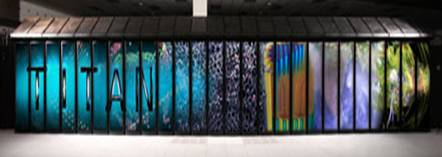
\includegraphics[height=0.75in,clip]{../figs/Titan}
    \end{figure}
 	\end{center}
 	
 	\alert{Architecture} influences algorithm choices and data management
	
\end{frame}

%%%%%%%%%%%%%%%%%%%%%%%%%%%%%%%%%%%%%%%%%%%%%%%%%%%%%%
%%%%%%%%%%%%%%%%%%%%%%%%%%%%%%%%%%%%%%%%%%%%%%%%%%%%%%
\begin{frame}{MC on GPU: WARP \cite{warp}}
	\begin{itemize}
	\item{Weaving All the Random Particles}
	\pause
	\item{Originally developed by Dr. Ryan Bergmann; current development by Kelly Rowland}
	\pause
	\item{3D continuous-energy Monte Carlo neutron transport code developed
	     for efficient implementation on \alert{GPUs}}
	\item{Can calculate multiplication factors, flux tallies, fission source
	     distributions for steady-state problems}
	\item{Run in either criticality or fixed-source mode}
	\item{Permits unrestricted arrangements of parallelpipeds, hexagonal prisms, 
	     cylinders, spheres}
	\pause
	\item{Now developing \alert{delta tracking} \cite{woodcock}}
	\end{itemize}
\end{frame}

%------------------------------------------------------
\begin{frame}{WARP's Demonstrated Success}
 
    \begin{center}
 	\begin{figure}     
 	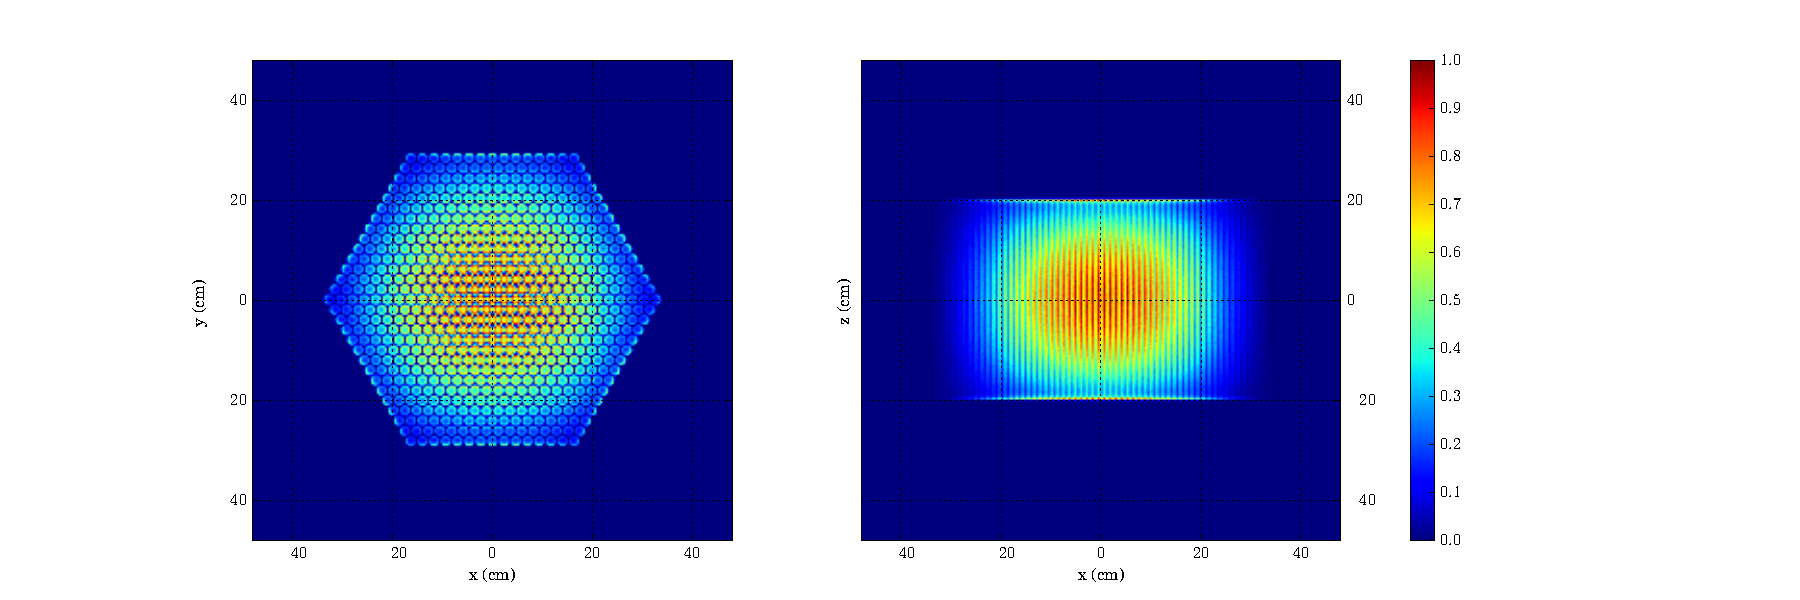
\includegraphics[height=1.5in,clip]{../figs/assembly-fiss-6}
 	\end{figure}
 	\end{center}   
 	
 	\begin{center}
 	\begin{figure}     
 	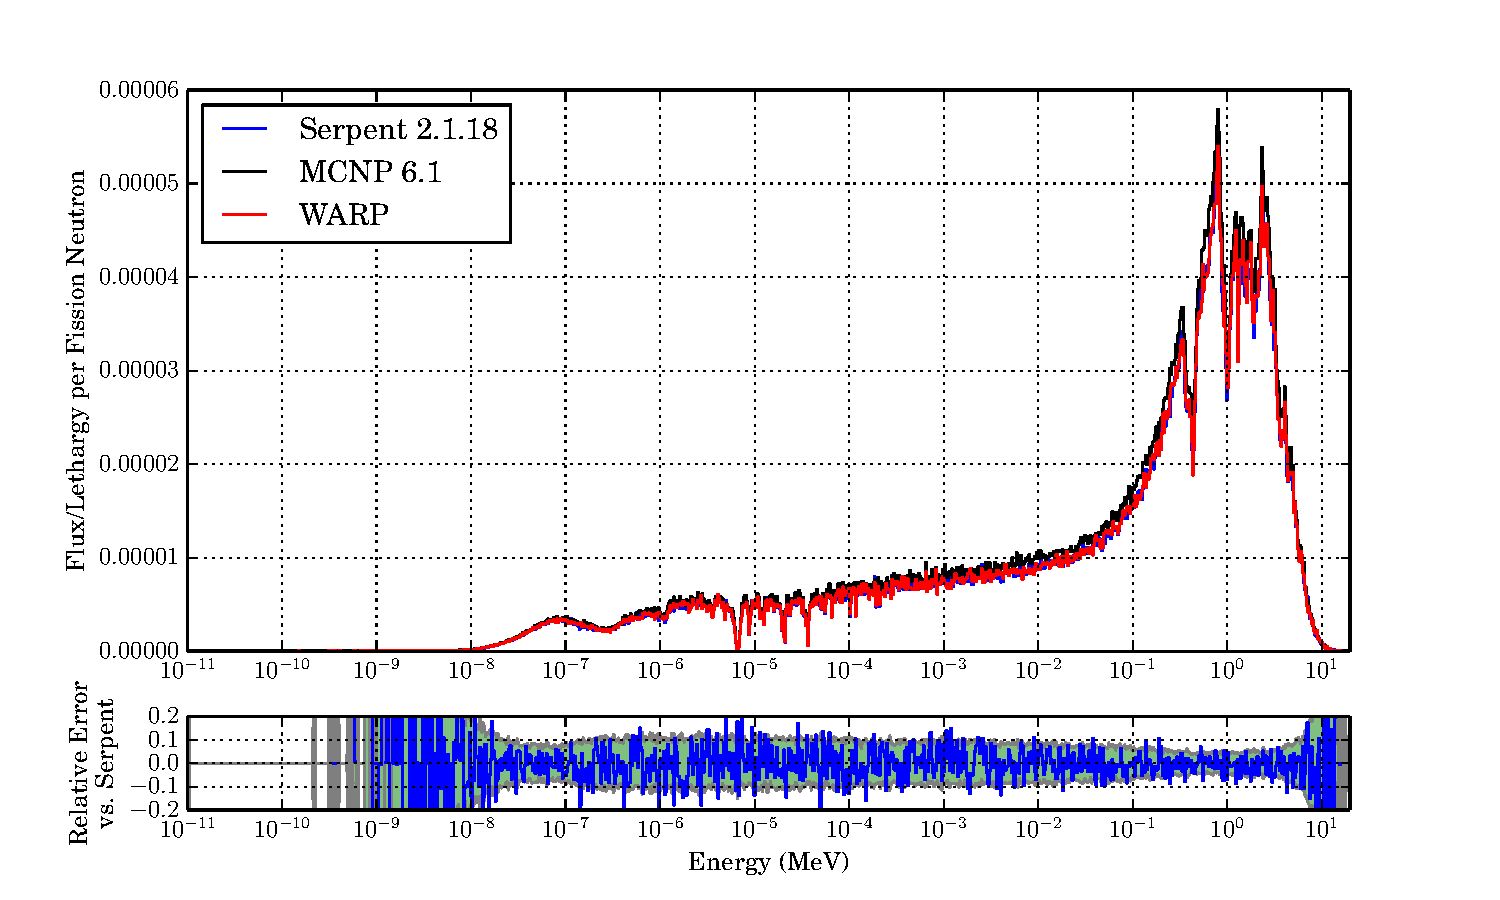
\includegraphics[height=1.5in,clip]{../figs/assembly-spec-6}
 	\end{figure}
 	\end{center} 
 
\end{frame}

%%%%%%%%%%%%%%%%%%%%%%%%%%%%%%%%%%%%%%%%%%%%%%%%%%%%%%
%%%%%%%%%%%%%%%%%%%%%%%%%%%%%%%%%%%%%%%%%%%%%%%%%%%%%%
\begin{frame}[fragile]
  \frametitle{Deterministic Scaling and Performance}

	\begin{columns}
  	\begin{column}{0.5\textwidth}
     \begin{itemize}
     \item Collaboration with deterministic code, \alert{Denovo} \cite{Evans2010} 
     \item Methods in Denovo scale very well using
       \begin{itemize}
       \item Krylov solvers, 
       \item optimized communication, and 
       \item parallelization in energy
       \end{itemize}
       \vspace*{1 em}
     \item Basic methods research tools being developed in \alert{PyNE} \cite{pyne2014}
     \end{itemize}
  	\end{column}
 	%
 	\begin{column}{0.5\textwidth}
 	 \begin{center}
 	 \begin{figure}
 	 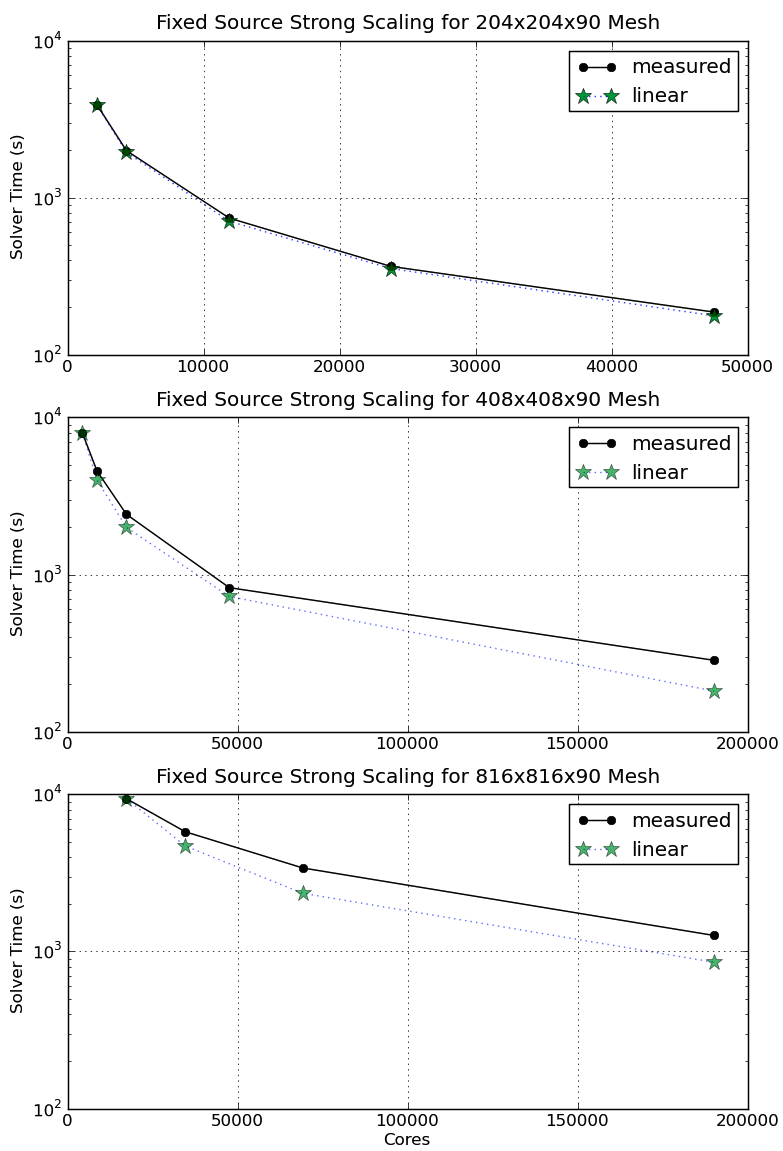
\includegraphics[height=3 in,clip]{../figs/FxdSrcKrylovStrongScaling}  
 	 \end{figure}
 	 \end{center}
  	\end{column}
	\end{columns}

\end{frame}

%%%%%%%%%%%%%%%%%%%%%%%%%%%%%%%%%%%%%%%%%%%%%%%%%%%%%%
%%%%%%%%%%%%%%%%%%%%%%%%%%%%%%%%%%%%%%%%%%%%%%%%%%%%%%
\begin{frame}[fragile]
  \frametitle{Hybrid Methods are Insufficient for Non-Proliferation Work}

	\begin{itemize}
	\item MC VR parameters created from adjoint deterministic flux that is a
	      function of \emph{space and energy only}
	\item Angular dependence of the importance function is not retained, otherwise
	      the map would be
	  \begin{itemize}
	  \item very large (tens or hundreds of GB)
	  \item more costly and complex to use in MC simulation
      \end{itemize}	   
      \vspace*{1 em}
	\item Drawback: within a given space/energy cell, the map provides the
	      \emph{average} importance of a particle moving in \emph{any direction}
	      through the cell -- excluding information about how particles move
	      \underline{toward} the objective
	\end{itemize}

\end{frame}

% --------------------------------------------------------------
\begin{frame}[fragile]
  \frametitle{Example Inefficient VR Map \cite{Peplow2012}}

	\begin{columns}
  	\begin{column}{0.5\textwidth}
 	 \begin{center}
 	 \begin{figure}
 	 \includegraphics[height=2in,clip]{../figs/boat-interrogation}  
 	 \caption{Spherical boat model with source on left and fissionable material at center}
 	 \end{figure}
 	 \end{center}
  	\end{column}
 	%
 	\begin{column}{0.5\textwidth}
 	 \begin{center}
 	 \begin{figure}
 	 \includegraphics[height=2in,clip]{../figs/boat-map}  
 	 \caption{Target CADIS weight window values for 14.1 MeV neutrons}
 	 \end{figure}
 	 \end{center}
  	\end{column}
	\end{columns}

\end{frame}

% --------------------------------------------------------------
\begin{frame}[fragile]
  \frametitle{New, Angle-Informed Hybrid Methods in Development}

	\begin{itemize}
	\item Using new integration strategy to get scalar flux for use in 
	      FW-CADIS \cite{Peplow2012}
	\item Implementing LDO method \cite{Ahrens2014} in Denovo
	  \begin{itemize}
	  \item Re-derivation of $S_N$ with an interpolatory quadrature framework
	  \item Allows evaluation at directions not on quadrature set
	  \item No need to store spherical harmonic moments
	  \item May be useful for more accurately capturing strong anisotropies
	  \end{itemize}
	\end{itemize}
	
	\begin{center}
 	\begin{figure}
 	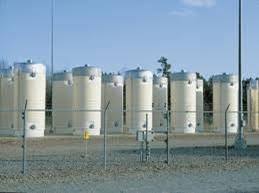
\includegraphics[height=1in,clip]{../figs/isfsi}
    \end{figure}
 	\end{center}

\end{frame}

%%%%%%%%%%%%%%%%%%%%%%%%%%%%%%%%%%%%%%%%%%%%%%%%%%%%%%
%%%%%%%%%%%%%%%%%%%%%%%%%%%%%%%%%%%%%%%%%%%%%%%%%%%%%%
\begin{frame}[fragile]
  \frametitle{Advanced Methods for HPC in Non-Proliferation}

	\begin{itemize}
	\item summary slide
	\end{itemize}

\end{frame}

% --------------------------------------------------------------
\begin{frame}[fragile]{Questions?}

    \begin{center}
    \includegraphics[height=3in,clip]{../questions-comic}  
    \end{center}
  
\end{frame}

% --------------------------------------------------------------
\begin{frame}[allowframebreaks]{References}
	\bibliographystyle{unsrt}
	\bibliography{hpc-highlevel.bib}
\end{frame}

\end{document}
